\documentclass{beamer}


\usetheme{AnnArbor}
\usecolortheme{default}


\title{The Art Of the Puzzle}
%\subtitle{Complex Systems Engineering}
\author{Steve Mazza}
\institute[Naval Postgraduate School]
{ 
    Naval Postgraduate School \\
    Monterey, CA \\
    
\includegraphics[height=3cm]{images/NPS_logo.jpg}
}
\date {SE4920, Summer/2014}
\subject{Reverse Engineering}


\begin{document}

\frame{\titlepage}


\frame{{Introduction}
  \begin{block}{Sam Loyd}
    ``I have always treated and considered puzzles from an educational standpoint. \dots[They] sharpen the wits, clear fog and cobwebs from the brain, and school the mind to concentrate properly.''
  \end{block}
  \begin{block}{Will Shortz}
    ``Of course, puzzles are designed primarily for entertainment.  That's why we do them.  But it's nice to know that we're becoming smarter and better human beings in the process.''
  \end{block}
}

\frame{{Puzzles, Science, and Mathematics}
  \begin{itemize}
    \item Mathematics is the solving of abstract puzzles
    \item Feynman attributed some of his contributions to quantum mechanics to his lifelong passion for puzzle solving.\footnote{Feynman also like safe cracking, a form of puzzle solving}
    \item topology and graph theory have their origins in Euler's puzzle about the Bridges of K{\"o}nigsberg.
  \end{itemize}
}
\frame{{Puzzles and Life}
  \begin{itemize}
    \item Puzzles reflect the mentality of their times.
    \item They reflect the
      \begin{itemize}
        \item Culture
        \item Values
        \item History
        \item Society
      \end{itemize}
  \end{itemize}
}
\frame{{Mechanical Puzzle Classification}
  Classifications are based on what must be done in order to solve the puzzle.
  \begin{enumerate}
    \item Put-together puzzles: put some object together.
    \item Take-apart puzzles: opening or taking apart the puzzle.
    \item Interlocking puzzles: involved disassembly or re-assembly.
    \item Disentanglement puzzles: disentangle or re-entangle the puzzle.
    \item Sequential-movement puzzles: move parts of the object to a goal.
    \item Dexterity puzzles: requires manual dexterity.
    \item Puzzle vessels: avoid spilling, or figure how to fill.
    \item Vanish puzzles: explain a vanished or changed image.
    \item Folding puzzles: fold the puzzle to form a specific pattern.
    \item Impossible puzzles: explain how a puzzle is made or why it behaves in a seemingly impossible way.
  \end{enumerate}
}
\frame{{Put-Together Puzzles}
  \begin{itemize}
    \item Solved by assembly
    \item The oldest class of mechanical puzzle
    \item Excellent example is the Tangram
  \end{itemize}
  \centering{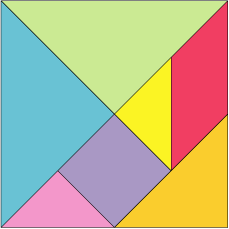
\includegraphics[scale=0.5]{images/Tangram.png}}
}
\frame{{Take-Apart Puzzles}
  Japanese puzzle boxes are an excellent example of these.  Many demonstrate various principles in physics.

  \centering{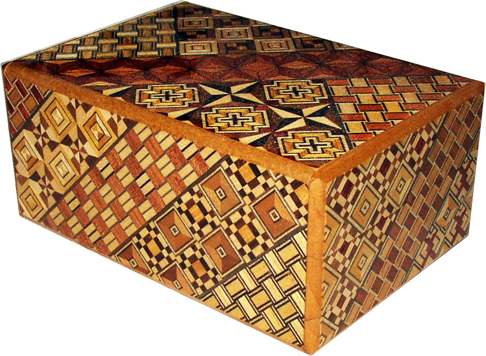
\includegraphics[scale=0.4]{images/puzzleBox.jpg}}
}
\frame{{Interlocking Puzzles}
  \begin{itemize}
    \item Often the greater challenge is in re-assembly
    \item Burr puzzles are representative of this type.
  \end{itemize}

  \centering{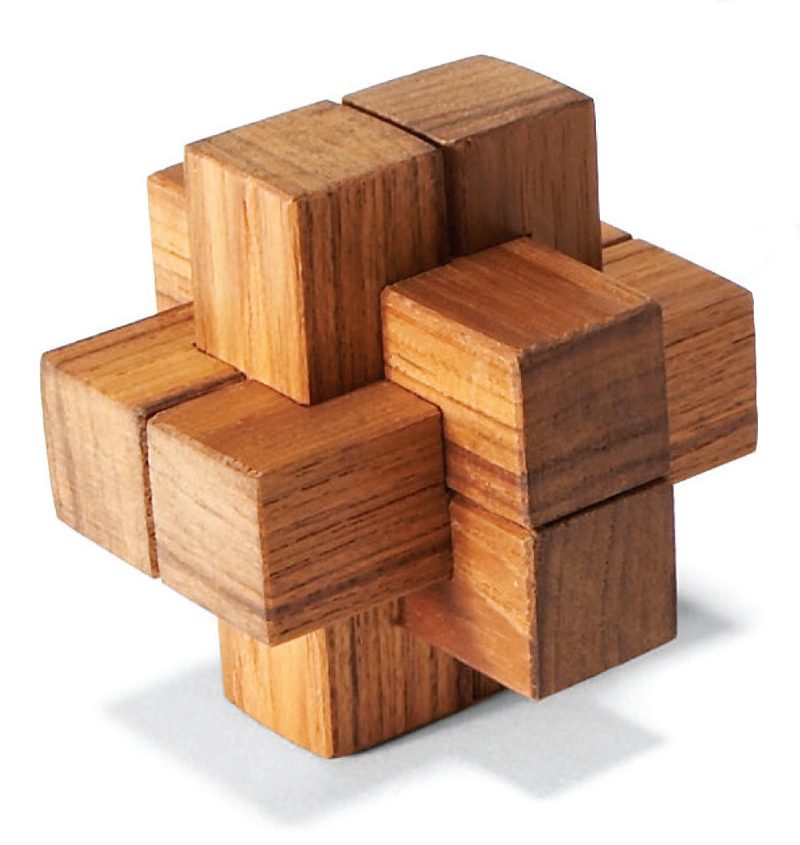
\includegraphics[scale=0.2]{images/burr.jpg}}
}
\frame{{Disentanglement Puzzles}
  \begin{itemize}
    \item Often involve freeing an attached part of the puzzle
    \item Examples include
      \begin{itemize}
        \item Solomon's Seal
        \item Chinese rings
        \item Hobble
      \end{itemize}
  \end{itemize}

  \centering{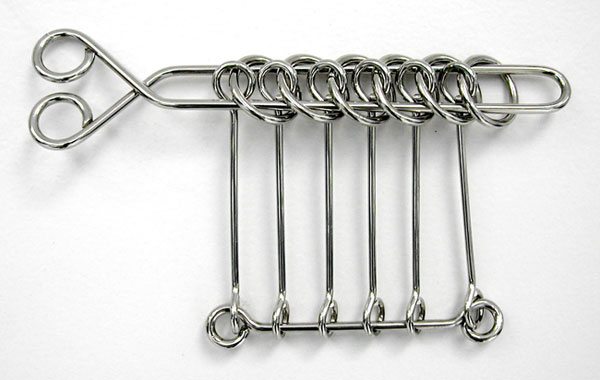
\includegraphics[scale=0.25]{images/chineseRings.jpg}}
}
\frame{{Sequential Movement Puzzles}
  \begin{itemize}
    \item Involve moving parts of a puzzle to a goal
    \item Examples include
      \begin{itemize}
        \item Puzzle of fifteen (sliding block puzzles)
        \item Rubik's Cube
      \end{itemize}
  \end{itemize}

  \centering{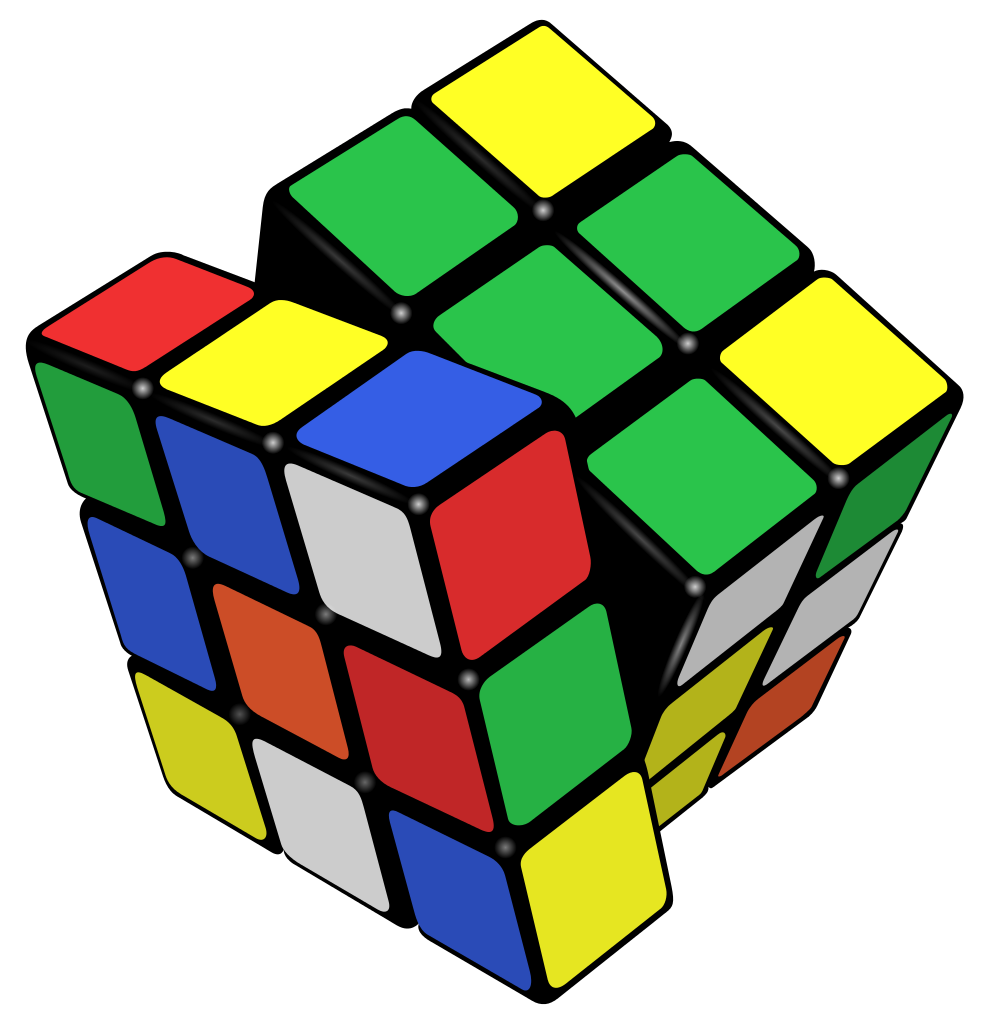
\includegraphics[scale=0.1]{images/rubik.png}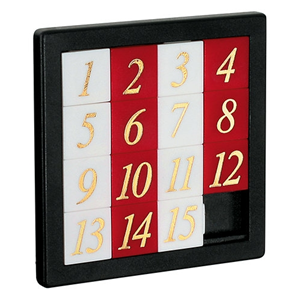
\includegraphics[scale=0.3]{images/fifteen.jpg}}
}
\frame{{Dexterity Puzzles}
  \begin{itemize}
    \item Throw and catch puzzles and rolling balls (in maze)
    \item Logic is often part of the key to the solution
    \item Specific type was used to help British prisoners escape during WWII
  \end{itemize}

  \centering{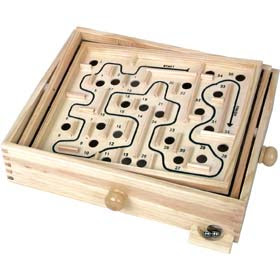
\includegraphics[scale=0.5]{images/marblemaze.jpg}}
}
\frame{{Puzzle Vellels}
  \begin{itemize}
    \item May require the solver to not spill while drinking
    \item Solutions involve using the vessel in other than ordinary ways
  \end{itemize}

  \centering{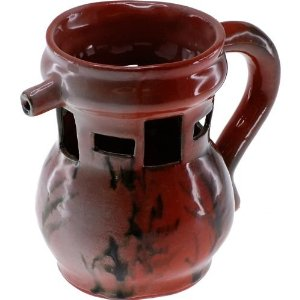
\includegraphics[scale=0.5]{images/vessel.jpg}}
}
\frame{{Vanish Puzzles}
  \begin{itemize}
    \item Geometric paradoxes
    \item Involve rearrangement of parts of a figure
    \item Part of the figure vanishes
    \item Examples include
      \begin{itemize}
        \item The Magic Egg
        \item Get Off the Earth
      \end{itemize}
  \end{itemize}

  \centering{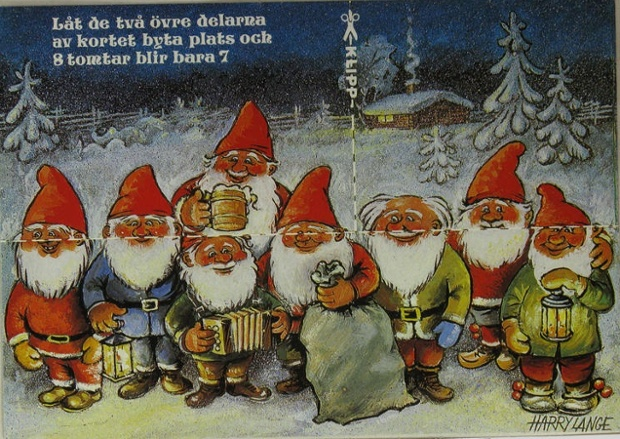
\includegraphics[scale=0.25]{images/magicegg.jpg}}
}
\frame{{Folding Puzzles}
  \begin{itemize}
    \item Have been used in advertisements
    \item Popular in Mad Magazine
  \end{itemize}

  \centering{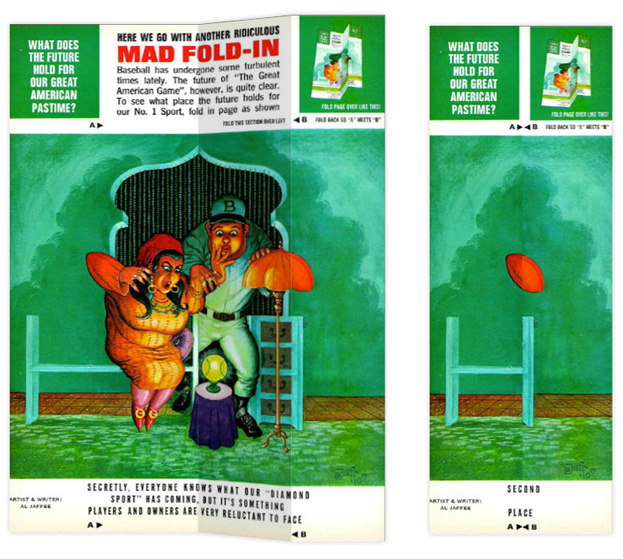
\includegraphics[scale=0.3]{images/jaffee.jpg}}
}
\frame{{Impossible Puzzles}
  \begin{itemize}
    \item Trick is to figure out how it was made
    \item Often include objects in bottles
  \end{itemize}

  \centering{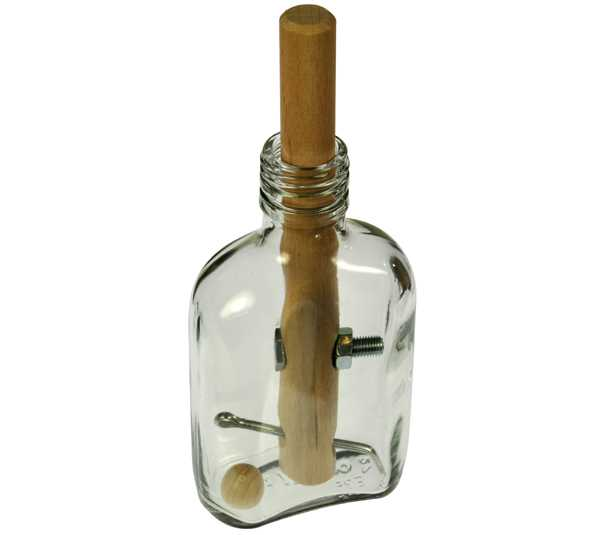
\includegraphics[scale=0.4]{images/bottle.jpg}}
}
\frame{{Summary}
  Puzzles
  \begin{itemize}
    \item Entertain
    \item Educate
    \item Protect
    \item Are art
    \item Require astute problem solving skills, analysis, and observation
  \end{itemize}
}

\end{document}
